\section{Les éléments du langage}

	\subsection{Types primitifs}
	
		\begin{frame}
			\frametitle{Les éléments du langage}
			\framesubtitle{Types primitifs}
			Tableau des types primitifs:
			\begin{center}
				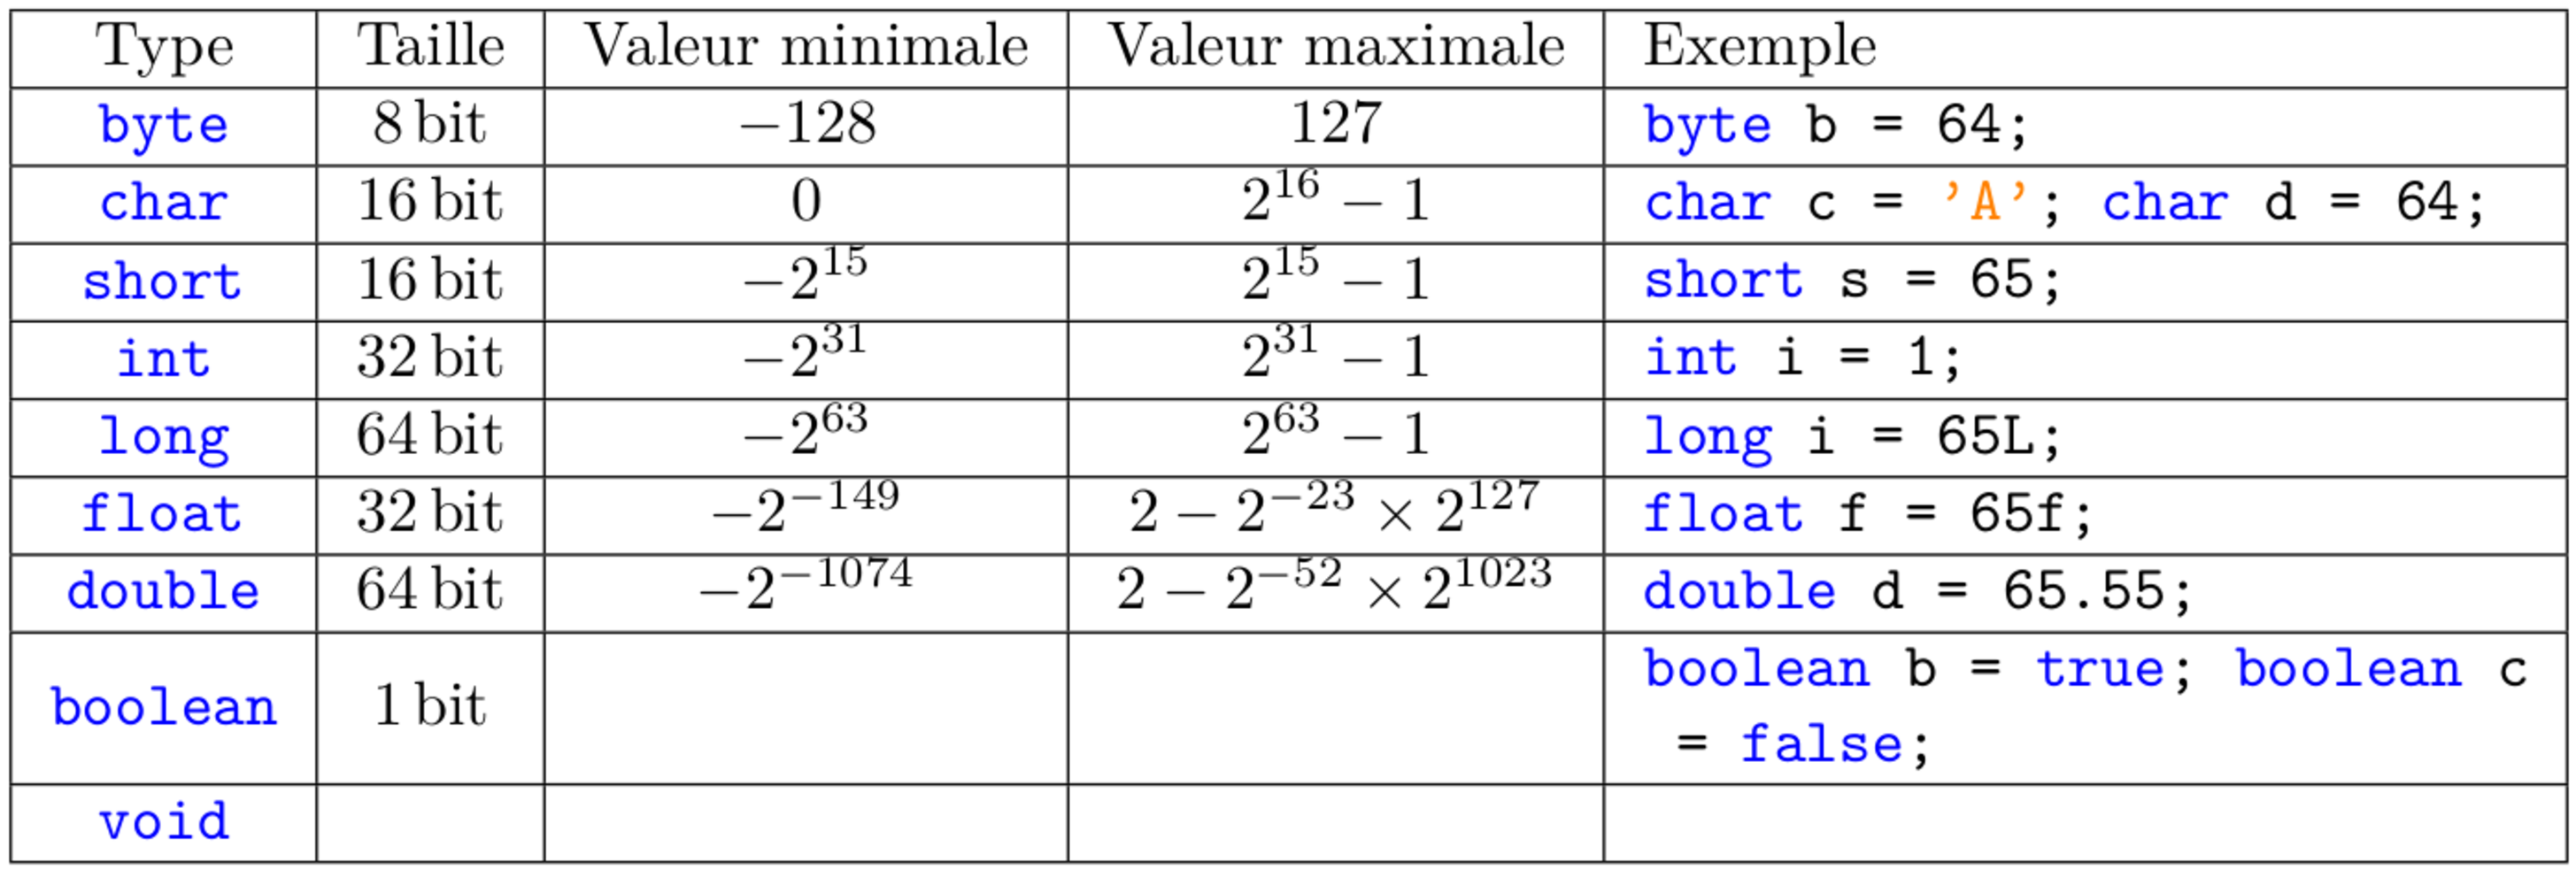
\includegraphics[width=1.0\linewidth]{images/typesprimitifs}
			\end{center}
		\end{frame}
			
	
	\subsection{Variables}
	
		\begin{frame}[fragile]
			\frametitle{Les éléments du langage}
			\framesubtitle{Variables}
			\begin{fact}
				En Java, les variables sont typées, et peuvent être déclarées dans n'importe quel bloc du code.
			\end{fact}
			\pause{}
			\begin{columns}
				\begin{column}{0.45\textwidth}
					\begin{example}
						\lstinputlisting{code/porteevariables.java}
					\end{example}
				\end{column}
				\begin{column}{0.45\textwidth}
					\pause{}
					\begin{block}{Résultat}
						La variable \lstinline|x| sera utilisable dans \visible<4->{\textcolor{purple}{les blocs 1 et 2}.}
						
						La variable \lstinline|y| sera utilisable \visible<5->{\textcolor{purple}{uniquement dans le bloc 2}.}
					\end{block}
				\end{column}
			\end{columns}
		\end{frame}
	
		\begin{frame}[fragile]
			\frametitle{Les éléments du langage}
			\framesubtitle{Variables}
			
			\begin{block}{Opérateurs d'affectation}
				\begin{itemize}
					\item \lstinline|=|
					\item \lstinline|+=|
					\item \lstinline|-=|
					\item \lstinline|*=|
					\item \lstinline|/=|
					\item \lstinline|%=|
				\end{itemize}
			\end{block}		
		\end{frame}
	
	\subsection{Expressions}
	
		\begin{frame}[fragile]
			\frametitle{Les éléments du langage}
			\framesubtitle{Expressions}
			\begin{definition}
				Une \emph{expression ternaire} est une notation \og simplifiée\fg{} d'un \emph{test logique}.
			\end{definition}
			\begin{columns}
				\begin{column}{0.45\textwidth}
					\pause{}
					\begin{example}[Test classique]
						\lstinputlisting{code/testClassique.java}
					\end{example}
				\end{column}
				\begin{column}{0.45\textwidth}
					\pause{}
					\begin{example}[Test ternaire]
						\lstinputlisting{code/operateurTernaire.java}
					\end{example}
				\end{column}
			\end{columns}	
		\end{frame}
	
		\begin{frame}[fragile]
			\frametitle{Les éléments du langage}
			\framesubtitle{Expressions}
			\begin{alertblock}{Attention !}
				Il est nécessaire de \emph{caster} des affectations lorsque celles-ci ne sont pas implicites, sinon des erreurs de compilation sont détectées.
			\end{alertblock}
			\pause{}
			\begin{example}
				\lstinputlisting{code/cast.java}
			\end{example}
			
		\end{frame}
	
		\begin{frame}[fragile]
			\frametitle{Les éléments du langage}
			\framesubtitle{Expressions}

			\begin{remarque}
				Levé d'ambiguité entre \lstinline|float| et \lstinline|double|:
				\lstinputlisting{code/floatdouble.java}
			\end{remarque}
		\end{frame}
	
	\subsection{Méthodes}
	
		\begin{frame}[fragile]
			\frametitle{Les éléments du langage}
			\framesubtitle{Méthodes}
			
			\begin{definition}
				Une \emph{méthode} est une fonction appartenant à une classe.
			\end{definition}
			\pause{}
			\begin{syntaxe}
				\lstinputlisting{code/basemethode.java}
			\end{syntaxe}
		\end{frame}
	
		\begin{frame}[fragile]
			\frametitle{Les éléments du langage}
			\framesubtitle{Méthodes}
			
			\begin{remarque}
				\begin{enumerate}
					\item \uncover<2,5->{Le type de retour est un type primitif, une classe ou \lstinline|void|.}
					\item \uncover<3,5->{La liste des paramètres peut être vide.}
					\item \uncover<4,5->{Si le type de retour n'est pas un \lstinline|void|, la fonction doit se terminer par un \lstinline|return|.}
				\end{enumerate}
			\end{remarque}
			\uncover<5->{
				Passage de paramètres:
				\begin{description}
					\item[Type simple:] passés \emph{par valeur} \alert{uniquement}
					\item[Type objet ou tableaux:] passés \emph{par référence}
				\end{description}
			}
		\end{frame}
	
	\subsection{Structures de contrôle}
	
		\begin{frame}[fragile]
			\frametitle{Les éléments du langage}
			\framesubtitle{Structures de contrôle (IF)}
			\begin{fact}
				Le code à l'intérieur d'un \lstinline|if| s'exécute uniquement si la condition est vraie.
			\end{fact}
			\pause{}
			\begin{alertblock}{Attention !}
				Plusieurs notations sont possibles ! Soyez vigilants au nombre de lignes de code dans votre bloc d'instructions (si votre condition est vraie) pour bien choisir la notation.
			\end{alertblock}
			\pause{}
			\begin{syntaxe}
				\begin{itemize}[<+->]
					\item \lstinline|if(condition) {...} else {...}|
					\item \lstinline|if(condition) instruction;|
					\item \lstinline|if(condition) instruction; else instruction;|
					\item \lstinline|if(condition) instruction; else {...}|
					\item \lstinline|if(condition) {...} else instruction;|
				\end{itemize}
			\end{syntaxe}
		\end{frame}
	
		\begin{frame}[fragile]
			\frametitle{Les éléments du langage}
			\framesubtitle{Structures de contrôle (IF)}
			\begin{example}
				\lstinputlisting{code/exempleIF.java}
			\end{example}
		\end{frame}
	
		\begin{frame}[fragile]
			\frametitle{Les éléments du langage}
			\framesubtitle{Structures de contrôle (WHILE)}
			\begin{fact}
				Le code à l'intérieur d'un \lstinline|while| s'exécute tant que la condition est vraie.
			\end{fact}
			\pause{}
			\begin{syntaxe}
				\begin{itemize}
					\item \lstinline|while(condition) {...}|
					\item \lstinline|while(condition) instruction;|
				\end{itemize}
			\end{syntaxe}
			\pause{}
			\begin{example}
				\lstinputlisting{code/exempleWHILEsansDO.java}
			\end{example}
		\end{frame}
	
		\begin{frame}[fragile]
			\frametitle{Les éléments du langage}
			\framesubtitle{Structures de contrôle (WHILE)}
			\begin{remarque}
				Le \lstinline|while|, tel que définit jusqu'à présent, vérifie la condition avant d'exécuter (au moins une fois) les instructions. 
				
				Dans certains cas, il peut être utilise d'exécuter les instructions au moins une fois, avant de vérifier si il faut les répéter.
			\end{remarque}
			\pause{}
			On utilisera l'instruction: \lstinline|do|.
			\pause{}
			\begin{syntaxe}
				\lstinline|do{ ... } while(condition)|
			\end{syntaxe}
			
		\end{frame}
	
		\begin{frame}[fragile]
			\frametitle{Les éléments du langage}
			\framesubtitle{Structures de contrôle (DO ... WHILE)}
			\begin{example}
				\lstinputlisting{code/exempleWHILEavecDO.java}
			\end{example}
			\pause{}
			\begin{remarque}
				Sans l'instruction \lstinline|do|, aucune instruction ne se serait exécutée.
			\end{remarque}
			
		\end{frame}
	
		\begin{frame}[fragile]
			\frametitle{Les éléments du langage}
			\framesubtitle{Structures de contrôle (FOR)}
			\begin{fact}
				Le code à l'intérieur d'une boucle \lstinline|for| s'exécute un nombre défini de fois.
			\end{fact}
			\pause{}
			\begin{syntaxe}
				\begin{itemize}
					\item \lstinline|for(initialisation, condition, incrementation) { ... }|
					\item \lstinline|for(initialisation, condition, incrementation) instruction;|
				\end{itemize}
			\end{syntaxe}
			Avec:
			\pause{}
			\begin{description}[<+->]
				\item[initialisation:] initialisation de la / les variable(s) de boucle
				\item[condition:] la boucle sera répétée tant que la condition sera vraie
				\item[incrementation:] incrémente la variable de boucle
			\end{description}
			
		\end{frame}
	
		\begin{frame}[fragile]
			\frametitle{Les éléments du langage}
			\framesubtitle{Structures de contrôle (FOR)}
			\begin{example}
				\lstinputlisting{code/exempleFOR.java}
			\end{example}
			\pause{}
			\begin{alertblock}{Attention !}
				Ce programme affiche les nombres de 0 à 9, et non jusqu'à 10 !
			\end{alertblock}
		\end{frame}
	
		\begin{frame}[fragile]
			\frametitle{Les éléments du langage}
			\framesubtitle{Structures de contrôle (SWITCH)}
			\begin{definition}
				Un \lstinline|switch| est un bloc contenant une succession de tests. On peut le comparer à une succession de \lstinline|if|.
			\end{definition}
			\pause{}
			\begin{itemize}
				\item Structure très utile pour effectuer beaucoup de tests avec la même variable.
				\item Elle évite d'écrire un programme avec une succession de tests en \lstinline|if| qui utilisent \alert{la même} variable d'entrée. 
			\end{itemize}
			
		\end{frame}
	
		\begin{frame}[fragile]
			\frametitle{Les éléments du langage}
			\framesubtitle{Structures de contrôle (SWITCH)}
			\begin{syntaxe}
				\lstinputlisting{code/syntaxeSwitch.java}
			\end{syntaxe}
			
		\end{frame}
	
		\begin{frame}[fragile]
			\frametitle{Les éléments du langage}
			\framesubtitle{Structures de contrôle (BREAK et CONTINUE)}
			\begin{remarque}
				Il peut être utile:
				\begin{enumerate}
					\item <2-> d'arrêter une boucle avant sa fin
					\item <3-> de passer automatiquement à l'itération suivante sans exécuter les instructions qui suivent dans le bloc
				\end{enumerate}
			\end{remarque}
			\visible<4->{
				Pour cela, on utilisera respectivement les instructions suivantes:
				\begin{enumerate}
					\item <5->\lstinline|break;|
					\item <6->\lstinline|continue;|
				\end{enumerate}
			}
			
		\end{frame}